\input{../preamble.tex}

\lecturenumber{21}
\title{Locks}
\version{2.0.0}

\begin{document}
  \begin{frame}[plain, noframenumbering]
    \titlepage
  \end{frame}

	
	\begin{slide}
	
		\slidetitle{Recap From Yesterday}
		
		Concurrent access to a shared variable by multiple threads causes a data race.
		
		\leftspace Data race causes undefined behavior
		\medskip
		
		A lock provides mutual exclusion
		
		\leftspace critical regions appear atomic to concurrent threads.
		\bigskip
		
		\begin{minted}{c}
pthread_mutex_t lock = PTHREAD_MUTEX_INITIALIZER;

pthread_mutex_lock(&lock);
// protected code
pthread_mutex_unlock(&lock);
\end{minted}

	\end{slide}

	\begin{slide}
	
		\slidetitle{Example of \texttt{pthread} lock}
		\vspace{-5mm}
\begin{minted}{c}
#define NUM_ITERATIONS 100000
int counter = 0;
pthread_mutex_t lock = PTHREAD_MUTEX_INITIALIZER;
void *worker(void *arg) {
    for (int i = 0; i < NUM_ITERATIONS; ++i) {
        pthread_mutex_lock(&lock);
        counter++;
        pthread_mutex_unlock(&lock);
    }
}
int main(void){
    pthread_t t1, t2;
    pthread_create(&t1, NULL, worker, NULL);
    pthread_create(&t2, NULL, worker, NULL);
    pthread_join(t1, NULL); pthread_join(t2, NULL);
    printf("Final counter value: %d\n", counter);
    return 0;
}
\end{minted}

	
	\end{slide}
	
	\begin{slide}
	
		\slidetitle{You may need more than one lock}
		
		You can use one mutex for all shared data. Every thread must take the same lock before touching any of it.	
		
		\leftspace Scales very poorly
		\bigskip
		
		Or you can have each independent shared object (or field, or small group of fields) has its own mutex. 
		
		\leftspace A thread grabs only the lock(s) that protect the data it will use.	
	
	\end{slide}
	
	\begin{slide}
	
	
		\slidetitle{Granularity of Locks - Example}
		
		\vspace{3mm}
		
		\centering
		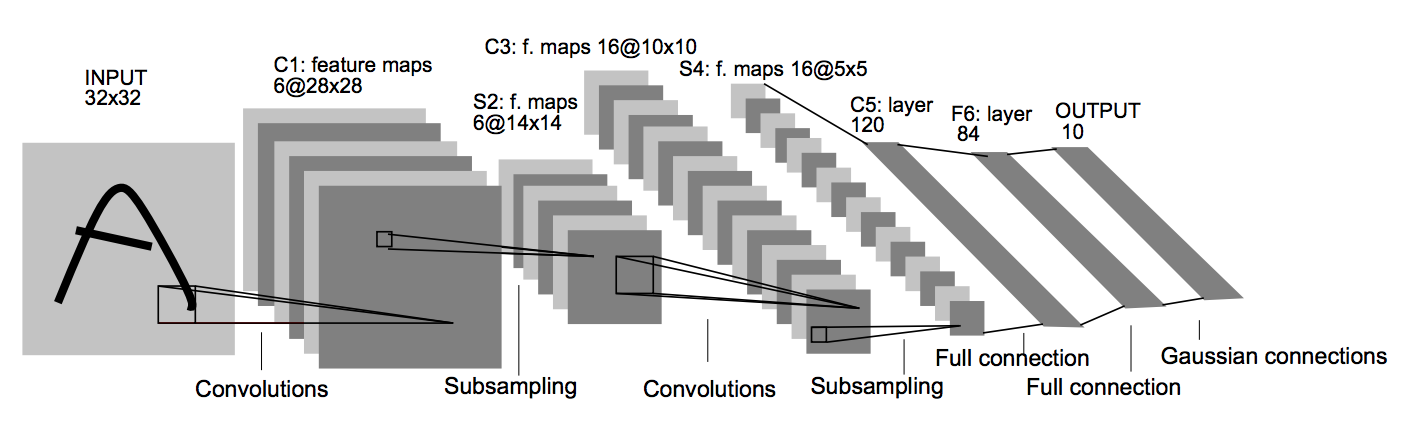
\includegraphics[width=120mm]{CNN-example.png}
		
	\end{slide}
	
	\begin{slide}
	
		\slidetitle{An example with two counters}
		
		\vspace{-5mm}
		
		\begin{minted}{c}
#define N_ITER 1000000
static long counterA = 0, counterB = 0;
static pthread_mutex_t lockA = PTHREAD_MUTEX_INITIALIZER;
static pthread_mutex_t lockB = PTHREAD_MUTEX_INITIALIZER;

void *incA(void *arg)
{
    for (int i = 0; i < N_ITER; ++i) {
        pthread_mutex_lock(&lockA);
        ++counterA;
        pthread_mutex_unlock(&lockA);        
        pthread_mutex_lock(&lockB);
        ++counterB;
        pthread_mutex_unlock(&lockB);
    }
    return NULL;
}
		\end{minted}
		
	
	\end{slide}
	
	
	\begin{slide}
	
		\slidetitle{What could happen with locks}
		\vspace{-5mm}
		
\begin{minted}{c}
pthread_mutex_t a = PTHREAD_MUTEX_INITIALIZER;
pthread_mutex_t b = PTHREAD_MUTEX_INITIALIZER;
int main() {
    pthread_t x, y;
    pthread_create(&x, NULL, t1, NULL);
    pthread_create(&y, NULL, t2, NULL);
    pthread_join(x, NULL);
    pthread_join(y, NULL);
    return 0;
}
\end{minted}
	\medskip
	\begin{minipage}{0.45\textwidth}
	\begin{minted}{c}
void* t1(void* _) {
    pthread_mutex_lock(&a);
    pthread_mutex_lock(&b);  
    pthread_mutex_unlock(&b);
    pthread_mutex_unlock(&a);
    return NULL;
}
\end{minted}
	\end{minipage}
	\hfill
	\begin{minipage}{0.45\textwidth}
	\begin{minted}{c}
void* t2(void* _) {
    pthread_mutex_lock(&b);
    pthread_mutex_lock(&a);  
    pthread_mutex_unlock(&a);
    pthread_mutex_unlock(&b);
    return NULL;
}
\end{minted}
	\end{minipage}
	
	\end{slide}

  \begin{slide}

    \slidetitle{A Critical Section Means Only One Thread Executes Instructions}

    Safety (aka mutual exclusion)

    \leftspace{}There should only be a single thread in a critical section at
    once
    \medskip

    Liveness (aka progress)

    \leftspace{}If multiple threads reach a critical section, one must proceed

    \leftspace{}The critical section can't depend on outside threads

    \leftspace{}\leftspace{}You can mess up and deadlock (threads don't make progress)
    \medskip

    Bounded waiting (aka starvation-free)

    \leftspace{}A waiting thread must eventually proceed

  \end{slide}

  \begin{slide}

    \slidetitle{Critical Sections Should Also Have Minimal Overhead}

    Efficient

    \leftspace{}You don't want to consume resources while waiting
    \medskip

    Fair

    \leftspace{}You want each thread to wait approximately the same time
    \medskip

    Simple

    \leftspace{}It should be easy to use, and hard to misuse

  \end{slide}

	\begin{slide}
	
		\slidetitle{How do we build a lock?}
		
		How can we build an efficient lock?
		
	\end{slide}
	
  \begin{slide}

    \slidetitle{You Could Use a Lock to Implement Critical Sections}

    Assuming a uniprocessor operating system, your implementation could be:
    \medskip

    \begin{minted}{c}
void lock() {
  disable_interrupts();
}
void unlock() {
  enable_interrupts();
}   
    \end{minted}
    \medskip

    This would disable concurrency (assuming it ignores signals and interrupts)

    \leftspace{}This does not work on multiprocessors

  \end{slide}

  \begin{slide}

    \slidetitle{Let's Try to Implement a Lock in Software}

    \begin{minted}{c}
void init(int *l) {
  *l = 0;
}
void lock(int *l) {
  while (*l == 1);
  *l = 1;
}
void unlock(int *l) {
  *l = 0;
}   
    \end{minted}
    \medskip

    \onslide<2->What's the issue with this implementation?

    \onslide<2->{\leftspace{}It's not safe (both threads can be in the critical section)}

    \onslide<2->{\leftspace{}It's not efficient, it wastes CPU cycles (busy wait)}

  \end{slide}

  \begin{slide}

    \slidetitle{Let's Assume a Magical Atomic Function ---
                \texttt{compare\_and\_swap}}

    \texttt{compare\_and\_swap(int *p, int old, int new)} is atomic

    \leftspace{}It returns the original value pointed to

    \leftspace{}It only swaps if the original value equals \texttt{old}, and changes it to \texttt{new}
    \medskip

    Let's give it another shot:

    \begin{minted}[xleftmargin=1em]{c}
void init(int *l) {
  *l = 0;
}
void lock(int *l) {
  while (compare_and_swap(l, 0, 1));
}
void unlock(int *l) {
  *l = 0;
}   
    \end{minted}

  \end{slide}

  \begin{slide}

    \slidetitle{What We Implement is Essentially a Spinlock}

    Compare and swap is a common atomic hardware instruction
    \medskip

    On x86 this is the \texttt{cmpxchg} instruction (compare and exchange)
    \medskip

    However, it still has this ``busy wait'' problem
    \medskip

    Consider a uniprocessor system, if you can't get the lock, you should yield

    \leftspace{}Let the kernel schedule another process, that may free the lock
    \medskip

    On a multiprocessor machine, you could try again

  \end{slide}

  \begin{slide}

    \slidetitle{Let's Add a Yield}

    \begin{minted}{c}
void lock(int *l) {
  while (compare_and_swap(l, 0, 1)) {
    thread_yield();
  }
}
    \end{minted}

    Multiple threads may be waiting on the same lock
    \medskip

    We have no control over who gets the lock next

    \leftspace{}We need to be able to reason about it (FIFO is okay)

  \end{slide}

  \begin{slide}

    \slidetitle{We Can Add a Wait Queue to the Lock}

    \begin{minted}{c}
void lock(int *l) {
  while (compare_and_swap(l, 0, 1)) {
    // add myself to the lock wait queue
    thread_sleep();
  }
}
void unlock(int *l) {
  *l = 0;
  if (/* threads in wait queue */) {
    // wake up one thread
  }
}
    \end{minted}
    \medskip

  \end{slide}

  \begin{slide}

    \slidetitle{Lost Wakeup Example}

	\vspace{-5mm}

    \begin{minted}[linenos]{c}
void lock(int *l) {
  while (compare_and_swap(l, 0, 1)) {
    // add myself to the wait queue
    thread_sleep();
  }
}
void unlock(int *l) {
  *l = 0;
  if (/* threads in wait queue */) {
    // wake up one thread
  }
}
    \end{minted}
    \medskip

    Assume we have thread 1 (T1) and thread 2 (T2), thread 2 holds the lock

    \leftspace{}T1 runs line 2 and fails, swap to T2 that runs lines 10-12, T1
    runs lines 3 -4

    \leftspace{}\leftspace{}T1 will never get woken up!
  \end{slide}

  \begin{slide}

    \slidetitle{Wrong Thread Getting the Lock Example}

	\vspace{-5mm}
	
    \begin{minted}[linenos]{c}
void lock(int *l) {
  while (compare_and_swap(l, 0, 1)) {
    // add myself to the wait queue
    thread_sleep();
  }
}
void unlock(int *l) {
  *l = 0;
  if (/* threads in wait queue */) {
    // wake up one thread
  }
}
    \end{minted}
    \medskip

    Assume we have T1, T2, and T3. T2 holds the lock, T3 is in queue.

    \leftspace{}T2 runs line 9, swap to T1 which runs line 2 and succeeds

    \leftspace{}\leftspace{}T1 just stole the lock from T3!
  \end{slide}

  \begin{slide}

	\vspace{-5mm}
	
    \slidetitle{We Can Use Two Variables to Fix This (One to Guard)}

    \begin{columns}
      \begin{column}{0.5\textwidth}
        \begin{minted}{c}
typedef struct { int lock; int guard;
                 queue_t *q; } mutex_t;

void lock(mutex_t *m) {
  while (
    compare_and_swap(m->guard, 0, 1)
  );
  if (m->lock == 0) {
    m->lock = 1; // acquire mutex
    m->guard = 0;
  } else {
    enqueue(m->q, self);
    m->guard = 0;
    thread_sleep();
    // wakeup transfers the lock here
  }
}
        \end{minted}
      \end{column}
      \begin{column}{0.5\textwidth}
        \begin{minted}{c}
void unlock(mutex_t *m) {
  while (
    compare_and_swap(m->guard, 0, 1)
  );
  if (queue_empty(m->q)) {
    // release lock, no one needs it
    m->lock = 0; 
  }
  else {
    // direct transfer mutex
    // to next thread
    thread_wakeup(dequeue(m->q));
  }
  m->guard = 0;
}
        \end{minted}
      \end{column}
    \end{columns}

  \end{slide}

  \begin{slide}

    \slidetitle{There's STILL A Data Race}

    After a thread calls \texttt{lock}, it could get interrupted right before
    the \texttt{thread\_sleep}
    \medskip

    However, it's been added to the wait queue, so \texttt{thread\_wakeup}

    would try to wake up a thread that's not sleeping yet (we know it's about
    to)
    \medskip

    We could simply retry the call to \texttt{thread\_wakeup}

    until the thread finally calls \texttt{thread\_sleep}

  \end{slide}


\end{document}
